\documentclass[12pt, a4paper]{report}
\usepackage {graphicx,booktabs, gensymb,amsmath,appendix}

\title{Study of multiple Heat Diffusion schemes through a C++ implementation}
\author{Yoann Masson \\ Student in Software Engineering at Cranfield University}
\date{5\textsuperscript{th} of december, 2017}

\graphicspath{{plot/}}
\begin{document}

\begin{titlepage}
\maketitle
\end{titlepage}


\begin{abstract}
This report is about studying 4 schemes to implement a numerical solution of the heat diffusion equation in a 1D material through time. The equation is given by the following formula: \begin{equation}\frac{\partial T}{\partial t} = D\frac{\partial^2T }{\partial x^2}
\end{equation} 
The constraint are the following, a one foot long wall at an initial temperature of 100\degree F is being subject to a rise of its surface temperature to 300\degree F. The diffusivity D of the material is 0.1ft\textsuperscript{2}/hr. We will study the rise of the temperature of the material with time t = { 0.0, 0.1, 0.2, 0.3, 0.4, 0.5}.
\\
We will see four different schemes, each of them is providing a numerical solution. Those schemes are split into two categories:
\begin{itemize}

\item explicit schemes, schemes where there is only one unknown in the equation making it eazier to implement but less acurate
\begin{itemize}
\item DuFort \& Frankel Method
\item Richardson Method
\end{itemize}
\item implicit schemes, schemes where there are mutiple unkowns that needs to be solved through a linear system, which is harder and more time consuming to solve, but are far more accurate.
\begin{itemize}
\item Laasonen Method
\item Crank \& Nicolson Method
\end{itemize}
\end{itemize}

The four methods will give four different solutions that we will compare with the known analytical solution. Firstly the discussion will be oriented toward the behaviour of the errors and secondly we will discuss about the C++ solution that I provided.
\end{abstract}


\tableofcontents


\chapter{The analytical solution}
\section{The expected behaviour}
By chance, the heat diffusion equation has been solved and we know the temperature at the given time \textit{t} and space \textit{x}, with the given formula: \begin{equation}
T = T_{sur} + 2(T_{in} - T_{sur})\sum_{1}^{\infty}e^{-D(m\pi/L)^{2}t}\frac{1-(-1)^{m}}{m\pi}sin(\frac{m\pi x}{L})
\end{equation}
If we  plot the result for the wanted times, which are from time = 0 to time = 0.5 with a 0.1 time step we get the following plot:
\begin{figure}[h]
\centering
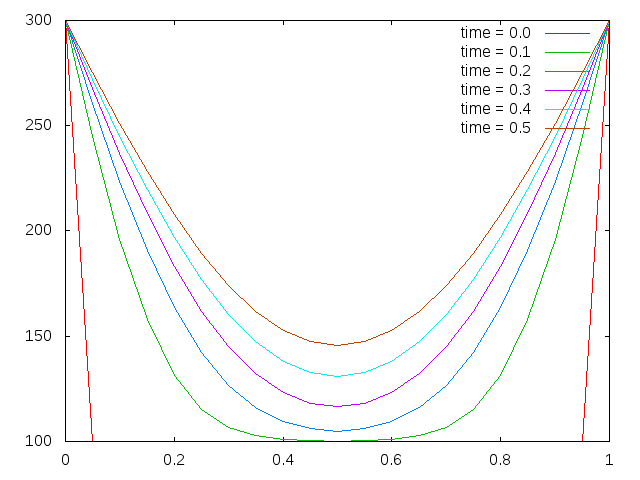
\includegraphics[scale=0.6]{Analytic.png}
\caption{Analytical solution}
\end{figure}
\\
As expected as the time flows the temperature is rising from the surface to the center. This is usefull to understand the heat diffusion behaviour. We will later use the data, used to make this plot, to compare with the other solution. This plot has been computed with a \textit{m} value of 50, which we will discuss in the next section.


\section{Study of \textit{m}}
\paragraph{}
\begin{equation}
\sum_{1}^{\infty}e^{-D(m\pi/L)^{2}t}\frac{1-(-1)^{m}}{m\pi}sin(\frac{m\pi x}{L})
\end{equation}
When considering the analytical equation of the heat diffusion, we can see that there is a sum to the infinty involving the term \textit{m}, which is of course not computable since we do not have an infinit time/space ressources to compute. In computer science, we can consider stopping the computation of the sum if the steps are becoming smaller and smaller, to the point where it is not use anymore to continue computing steps.
\paragraph{}
In this case, we are dealing with numbers in a range of 100 to 300, so I considered that an error less than 10\textsuperscript{-4} is acceptable. To know when the \textit{m} value is to be stopped I printed out the same time and space with different m value. Time is t = 0.01,0.25,0.5 and space is x = 0.5.
\begin{table}[ht]
\centering
\begin{tabular}{c c c c}
\toprule
\textit{m} value & temperature at t = 0.5 & temperature at t = 0.25 & temperature at t = 0.01 \\
\midrule
1 &144.5380&101.0325&47.8530\\
5 &145.5377&110.1387&85.7275\\
10 &145.5377&110.1389&95.4361\\
20 &145.5377&110.1389&100.1123\\
49 &145.5377&110.1389&100.0000\\
50 &145.5377&110.1389&100.0000\\
100 &145.5377&110.1389&100.0000\\
\end{tabular}
\caption{Temperature by \textit{m} value}
\end{table}\\
The outcome of those results is that in this example, we don't need such a high value for \textit{m}, we can see that values stop varying after \textit{m} > 49. If we want an error less than 10\textsuperscript{-4}, \textit{m} = 50 is enough. Thanks to that, we know that we don't have to waste computer ressources and time on computing the analytical solution with a higher \textit{m} value.


\chapter{Laasonen method,\\ time step size and computation time}

\section{Theory}
\paragraph{Laasonen method}
The Laasonen method is a way of solving the heat diffusion equation by computing a result step by step. The Laasonen method is part of the implicit scheme meaning that each time step not only relies on the previous one but also one the current one. When computing the result, the previous time step has already been computed but the current one will need to be solved through a linear system. Let's see the equation to get a clearer idea:
\begin{equation}\frac{\partial T}{\partial t} = D\frac{\partial^2T }{\partial x^2}
\end{equation} 
\begin{equation}\frac{f\binom{n+1}{i} - f\binom{n}{i}}{\Delta t} = D\frac{f\binom{n+1}{i+1} - 2f\binom{n+1}{i}+ f\binom{n}{i}}{\Delta x^{2}}
\end{equation} 
\begin{equation}f\binom{n}{i} = -Cf\binom{n+1}{i+1}+(1+2C)f\binom{n+1}{i}-Cf\binom{n+1}{i-1}
   \text{ with }
C = D\frac{\Delta t}{\Delta x^{2}}
\end{equation}
\begin{equation}
\begin{pmatrix}
1+2C & -C & 0 & ... & 0\\
-C & 1+2C & -C& ... & 0\\
...&...&...&...&...\\
 0 & ...& -C &1+2C & -C \\
0 & ... &  0& -C & 1+2C
\end{pmatrix}
\begin{pmatrix}
f\binom{n+1}{0}\\
f\binom{n+1}{1}\\
...\\
...\\
f\binom{n+1}{k}
\end{pmatrix}
=
\begin{pmatrix}
f\binom{n}{0}\\
f\binom{n}{1}\\
...\\
...\\
f\binom{n}{k}
\end{pmatrix}
\end{equation}
With the above equations, we can see that we need to solve a linear system for each time step. Linear system can be really time and ressources consumming for a computer. That's why we need a good algorithm to resolve this linear system, if we take a look at the left matrix we can see that it is a diagonal matrix.\\
A linear system with a diagonal matrix can be solved with Thomas' algorithm, which is a really good linear system solving algorithm that works with diagonal matrix, it's time complexity is of:  \textit{O(2n)} with n being the size of the matrix, so the number of space step we want, L=1 $\Delta$t=0.05 so we have 21 space steps. Meaning that a matrix twice larger will "only" take four time the requiered time.
\paragraph{}
Since the method relies on computing different time with a constant time step, a good interrogation would be: what is a good time step ? In theory, considering a stable method we can expect a more accurate solution the smaller the time step is.

\section{Pratice} 
Having a smaller and smaller difference between time steps allows us to have a better precision on each row, but if we decrease the time step we increase the number of linear system we need to solve. So I ran 4 simulations with various value of $\Delta$t, to compare the results. Let's see the norms of the errors matrices, the errors matrices is the Laasonen resulting matrix minus the analytical matrix:
\begin{table}[ht]
\centering
\begin{tabular}{c c c c c c}
\toprule
$\Delta$t&Number of time step&One norm&Two norm&uniform norm&computing time\\
\midrule
0.1 &5&50.26&67.01&154.56&0.14ms\\
0.05 &10&58.62&60.62&102.73&0.6ms\\
0.025 &20&67.90&52.13&64.04&0.42ms\\
0.01 &50&77.01&39.68&36.26&2.2ms\\
\end{tabular}
\caption{Error norms according to $\Delta$t}
\end{table} \\
Increasing the number of rows in the matrix by decreasing the time step size affects the one and two norms. Because the one norm is the highest error among the sums of error in each column and the two norm is just the sum of all errors. So more rows equals to possibly a worst one and two norms\\

\paragraph{one norm} The one norm is about errors in one column, so for $\Delta$t = 0.1, we can say that on average the "worst" column has an error of 50.26/5=10.05. Considering the fact that we are dealing with numbers in range of 100-300, this is almost a 10\% error on average. Compared to the $\Delta$t = 0.01 that has an average of 77.01/50 = 1.5 error, that's about 1\%error.\\
According to the one norm, decreazing the size of time steps is a good idea.

\paragraph{two norm} The two norm is just the square root of the sum errors, so increasing the numbers of rows in the matrix should increase the two norm, which is not the case. Between $\Delta$t = 0.1 and $\Delta$t = 0.05, we double the matrix size but the sum of errors is even smaller meaning that we have fewer errors overall.

\paragraph{uniform norm} The uniform norm is the highest number among the sum of rows. Increasing the number of rows does not affect the behaviour of this number, so if this decreases with a smaller time step size, it means that the method is more and more accurate. By comparing the worst uniform norm 154.56 and the best 36.26,  we can say that the worst row with a $\Delta$t = 0.1 is nearly six times less accurate than the worst row with a $\Delta$t = 0.01.

\paragraph{} On a stable method such as Laasonen we have clearly seen that having a smaller $\Delta$t is giving the method a better accuracy, going from 10\% to nearly 1\% error with the first norm. In an ideal case we should find the best deal between time computing and errors, not to forget that If we want to be very accurate we would hurt ourself against errors implied by the numerical 64-bit system.

\chapter{Methods Result}
\section{Unstable Method}
As we said already, thoses numerical schemes are based on computing steps after steps using the principe of derivatives. That is why, the more steps we have the more accurate results we have because the $\Delta$ in $f(x+\Delta x)$is smaller. This is introducing errors and we must be sure that the error are not comulating. In order to do this, we study the stability of the methods on the given problem. This means that every method does not work on every problem. Methods can be stable under certains conditions mostly relying on a $\Delta$x-$\Delta$t ratio. They can also be unconditionally stable/unstable meaning that for any $\Delta$x-$\Delta$t, the method will (or will not) work at any case.
\paragraph{Richardson case}
Let's take a look at Richardson method, it consists in derivating centrally the time and space.
\begin{equation}\frac{\partial T}{\partial t} = D\frac{\partial^2T }{\partial x^2}
\end{equation} 
\begin{equation}\frac{f\binom{n+1}{i} - f\binom{n-}{i}}{2\Delta t} = D\frac{f\binom{n+1}{i+1} - 2f\binom{n+1}{i}+ f\binom{n}{i}}{\Delta x^{2}}
\end{equation} 
\begin{equation}f\binom{n+1}{i} = Cf\binom{n}{i+1} - C2f\binom{n}{i}+ Cf\binom{n}{i-1})+f\binom{n-1}{i} \text{ with }
C = 2D\frac{\Delta t}{\Delta x^{2}}
\end{equation} 
Now that we have only one unknown we can figure it out. Since Richardson's method is unstable (see Appendix for proof) considering this problem, the results are not coherent at all.\\
\begin{figure}[h]
\centering
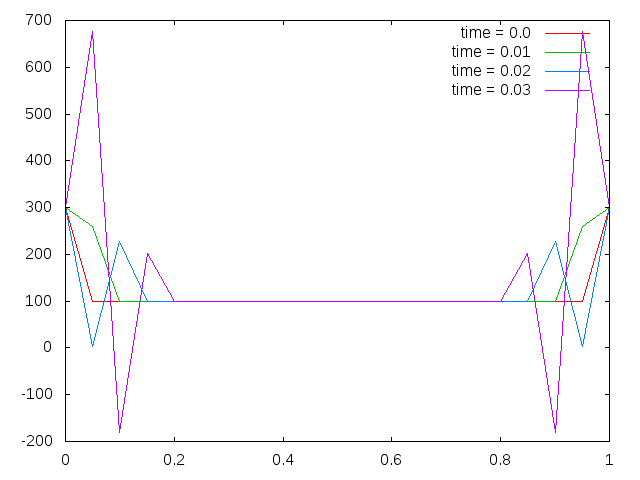
\includegraphics[scale=0.6]{Richardson.png}
\caption{Richardson solution}
\end{figure}
\paragraph{}
I only plotted the three first steps because it shows that with only three steps we can clearly see that the methods is incoherent. Temperatures are supposed to go in a range of 100\textsuperscript{o}F to 300\textsuperscript{o}F. Which is clearly not the case here.

\section{Stable Methods}
Within the conditions defined in the original problem, Dufort-Frankel Laasonen and Crank-Nic
holson methods are stable, which means that we do not have to fear for the errors to grow exponentially. We can even expected a better accuracy with time.
\paragraph{results}
The best way to compare the results are to compare the norms of their error matrix. For that, we can take a look at table 3.1 that compares the one norm , two norm, uniform norm and the computation time of the three methods.\\
\begin{table}[ht]
\centering
\begin{tabular}{c c c c c}
\toprule
Method & One norm & Two norm & Uniform norm & Computation time \\
\midrule
Crank Nicolson & 14.95 & 14.48 & 20.77 & 2.04ms\\
Laasonen &77.01&39.68&36.26&3.17ms\\
Dufort-Frankel & 85.61 & 74.47 & 82.82 & 0.93ms\\
\end{tabular}
\caption{Accuracy of stable methods}
\end{table}\\
Looking at those results, we can clearly see the superiority of the implicit methods ( Crank-Nicolson \& Laasonen ) over the Dufort-Frankel method. The norms in this table represents the sum of errors, so the fewer errors the best a method is, regarding the considered norm. However, the computation time for Dufort-Frankel is far better. Crank-Nicolson seems to be the better deal here: the sum of the error of the least accurate time step is 20\textsuperscript{o}F. So considering 21 space step, that's a 1\textsuperscript{o}F error by number in average, which is acceptable. The second norm of Crank-Nicolson (14.48) that somehow represents the error in the all result matrix is also the best.\\
The outcome of this table is that if we have enough time we should consider using Crank-Nicolson since it is the more accurate method but if if we don't have enough computation time we should consider using Dufort Frankel. Dufort Frankel is a bit less accurate but is way faster because its computation only requires solving one equation and not a linear system.

\chapter{Implementation}
Now that's we saw the theory and the results, let's take a look at the C++ implementation and the design of the application.
\paragraph{Class Diagram}
\begin{figure}[h]
\centering
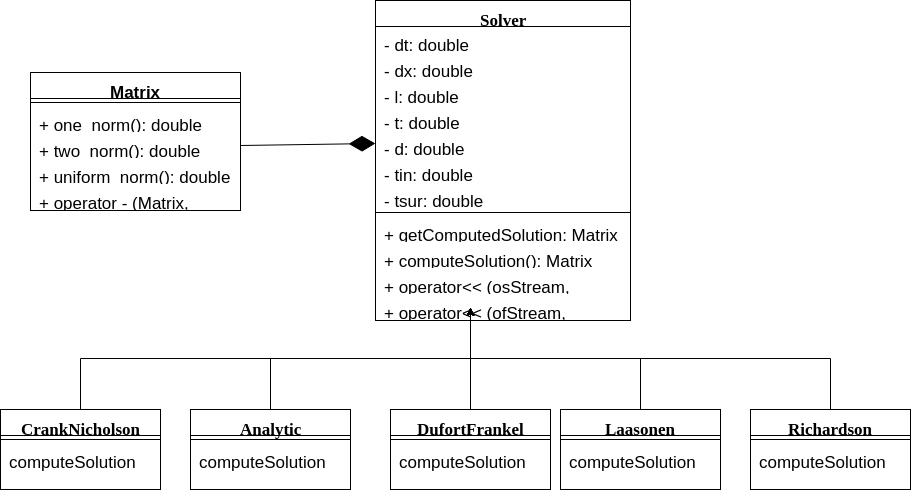
\includegraphics[scale=0.5]{ClassDiagram.png}
\caption{Class Diagramm}
\end{figure}
\begin{appendix}
\clearpage
\phantomsection
This is the class diagram of the application implementing the four schemes and the analytic solution.  The\textit{Solver} class uses \textit{Matrix} to store the solution of the problem where rows are time steps and columns are space steps. \textit{Solver} declares the virtual method \textit{computeSolution()} so that classes that inherit from it need to give an implementation of the solution for the  child class to be instanciated in a \textit{main} programm.\\
The base class \textit{Solver} class holds all of the informations regarding the initial problem. Since it is attribut and not just hard-coded value in the code, all the child class are bounded to those value. Let's say that we want to see the solution with a surface temperature of 250\textsuperscript{o}F instead of 300\textsuperscript{o}F, we just have to instanciate the object with a different \textit{Tsur} value.

\chapter{documentation}


\end{appendix}
\end{document}